\documentclass[11pt]{article}

\usepackage{dsfont}
\usepackage{amssymb}
\usepackage{mathtools}
\usepackage{geometry}
\geometry{a4paper}
\usepackage[parfill]{parskip}
\usepackage{graphicx}
\usepackage{amssymb}
\usepackage{epstopdf}
\usepackage{listings}
\lstset{language = C++}
\usepackage{url}

\newcommand{\re}[1]{\ensuremath{\operatorname{Re}(#1)}}
\newcommand{\im}[1]{\ensuremath{\operatorname{Im}(#1)}}

%\newcommand{\Vr}{\re{V}}
%\newcommand{\Vi}{\im{V}}
%\newcommand{\Ir}{\re{I}}
%\newcommand{\Ii}{\im{I}}
%\newcommand{\Sr}{\ensuremath{P}}
%\newcommand{\Si}{\ensuremath{Q}}

\newcommand{\Vr}{{V_R}}
\newcommand{\Vi}{{V_I}}
\newcommand{\Ir}{{I_R}}
\newcommand{\Ii}{{I_I}}
\newcommand{\Sr}{\ensuremath{P}}
\newcommand{\Si}{\ensuremath{Q}}

\newcommand{\Id}{\mathds{1}}

\title{Power Flow Theory}
\author{Dan Gordon}
\date{}

\begin{document}
\maketitle

\section{Nomenclature}
\begin{align*}
V &= \Vr + jW = \text{complex voltage.} \\
I &= \Ir + j\Ii = \text{complex current.} \\
S &= P + jQ = \text{complex power.} \\
y &= g + jb = \text{complex admittance} \\
Z &= R + jX = \text{complex impedance} \\
y_{ik} &= \text{complex admittance between busses $i$ and $k$.} \\
Y_{ik} &= G_{ik} + jB_{ik} = \text{nodal admittance matrix element $i, k$.} \\
\theta_{i} &= \text{the voltage angle of bus $i$.} \\
\theta_{ik} &= \theta_i - \theta_k = \text{the voltage angle difference between busses $i$ and $k$.} \\
I_{\text{ZIP},i} &= \text{total complex current injection from load at bus $i$.} \\
I_{\text{gen},i} &= \text{complex current injection due to the voltage controlled generation at bus $i$.} \\
S_{\text{gen},i} &= \text{complex power injection due to the voltage controlled generation at bus $i$.} \\
S_{ci} &= \text{constant power injection ZIP component of load at bus $i$.} \\
I_{ci} &= \text{constant current injection ZIP component of load.} \\
y_{ci} &= \text{constant impedance ZIP component of load.} \\
\delta_{ik} &= \text{the Kronecker delta, $\delta_{ik} = 1$ if $i = k$, 0 otherwise.}
\end{align*}

\section{The powerflow problem}
We start with a collection \emph{busses} -- terminal-like conductors that have a single associated voltage, $V_i$, where $i$ is the bus index. We can consider \emph{ground} to be a special bus (to which we assign index 0), at which $V$ is always zero.

Current can flow between busses, via the network. The current flowing from bus $i$ to $k$ is $I_{ik}$. 

Current that flows into a bus from ground is an \emph{injection} into the bus. We use the notation $I_{\text{inj},i} := I_{0i} = -I_{i0}$ to denote a current injection from ground to bus $i$. The power consumed as a result is $S_{0i} = I_{0i}^*(V_0 - V_i) = -I_{i}^*V_i$. The generated power -- that is, the power \emph{injection} into the bus -- is the negative of this: $S_{\text{inj},i} := I_{\text{inj},i}^*V_i$.

\emph{Kirchoff's current law} states that the total current flowing into a bus (from other busses and ground) is zero -- in other words, current in equals current out; electrical charges don't accumulate at busses. Thus
\begin{align}
	I_{i} - \sum_{k \ne i}{I_{ik}} &= 0
	\label{EQ_KCL}
\end{align}

The aim of the powerflow problem is, essentially, to find all bus voltages and currents\footnote{This will also trivially allow us to calculate power flows in the system -- we will discuss this later.}. To do so, we need to define the properties of the network to provide a functional relationship between current and voltage at the busses. We start with a simple formulation, where the current flow between any two busses is ohmic: it is defined by a fixed impedance between them. This describes a network of passive \emph{lines}. Later we will generalise this relationship, so that, for example, we can include transformers.

Suppose that $y_{ik} = y_{ki}$ is an impedance between busses $i$ and $k$. Then Ohm's law states that
\begin{align}
	I_{ik} &= y_{ik}(V_i - V_k)
\end{align}
Substituting this into KCL, Eq. (\ref{EQ_KCL}), gives
\begin{align}
	I_{\text{inj},i} - \sum_{k \ne i}{y_{ik}(V_i - V_k)} &= 0
	\label{EQ_PF_1}
\end{align}
which can be written as the matrix equation
\begin{align}
	I_\text{inj} - YV &= 0
\end{align}
where
\begin{align}
	Y_{ik} &=
		\begin{cases}
			-y_{ik}&\text{if $i \ne k$} \\
			\sum_{l \ne i} y_{il}& \text{if $i = k$}
		\end{cases}
	\label{EQ_YNODE_OHMIC}
\end{align}
However, in what follows, we do not make further use of the particular form of $Y$ expressed in Eq. (\ref{EQ_YNODE_OHMIC}) above. We simply require that $Y$ be a constant matrix, so that there is a linear relationship between $I$ and $V$. We shall see later that including components such as shunts and transformers allows us to retain the linear relationship while modifying the particular form of $Y$.

Due to the basic relation $S = I^*V$, the power loss between bus $i$ and $k$ is $S_{ik} = I_{ik}^*(V_i - V_k)$. Note that power is a scalar: if we reverse the order of the busses, then the power loss is unchanged, in contrast to, say, a current, where reversing the order of the busses will negate the current. More commonly, though, you will deal with the power entering or leaving a bus rather than the power lost in a line. Consider a current leaving a bus. If the current is a draw to ground, or if the system is radial and the current is in the direction of the downstream loads, all of this current will eventually end up at ground. The voltage drop in this process will just be the voltage of the bus. Thus, the power eventually transferred to ground will be 
\begin{align}
	S_\text{draw} = I_\text{draw}^*V_\text{bus}
\end{align}
or, equivalently, for injections
\begin{align}
	S_\text{inj} = I_\text{inj}^*V_\text{bus}
\end{align}
Note the way in which this concept of power is different to the concept of power loss in a line: the voltage in the equation is always the voltage of a bus relative to ground, and the current is always an injection or draw on a bus (rather than between two busses). There is an implied directionality: if the power draw from a bus is positive, then power is considered to be flowing from the bus to ground and we have a load.

The one piece of the puzzle we haven't yet dealt with is the current injections $I_\text{inj}$ into the busses. If the current injections were all constant, then the powerflow equations could be immediately solved by standard linear algebra. However, typically, the current injections from ground will depend on the bus voltage, and it is here that the real complexity of powerflow modelling comes into play.

Current injections take the form of \emph{loads} or \emph{generation}. Load currents can often be modeled using the \emph{ZIP} model:
\begin{align}
	I_\text{ZIP} = I_c + \frac{S^*_c}{V^*} - y_cV
\end{align}
Where $I_\text{ZIP}$ is the total current injection of the ZIP, $I_c$ and $S_c$ are constant current and power injections and $y_c$ is a constant impedance. The ZIP model is a good model for many types of load, but could also be used for certain types of generation - e.g. fixed power generation. If the real power injection $P = \re{I_\text{ZIP}^*V}$ is negative, then we have a load; if it is positive, then we have a generator.

In addition to the ZIP loads at a bus, we may include generators that apply some kind of extra voltage control on the bus to maintain power stability in the system. A bus that only has a ZIP load is termed a PQ bus. The term PQ means constant P, constant Q.\footnote{Confusingly, though, the presence of fixed current and fixed impedance components of the ZIP means that the total power injection may not be constant. This confusion arises because ZIP loads provide a generalisation to the original concept of PQ busses.}

We consider two other types of generator bus: SL (slack/swing/infinite/reference) busses, and PV busses. SL generators keep the total complex voltage of the bus fixed by injecting variable $P$ and $Q$. $PV$ busses keep the voltage magnitude $V$ and power $P$ fixed, while injecting a variable current\footnote{Note that the voltage angle is relative to the slack bus, and so is a non-local property of the network, hence it usually does not make sense to control it anywhere except at the slack bus.}. We write the additional generator current as a power $S_{gen}$ to simplify the later analysis.
\begin{align}
I_{gen} &= \frac{S_{gen}^*}{V^*}
\end{align}
Note that SL and PV busses may also have ZIP loads attached.

We now write the final form of the powerflow equations:
\begin{align}
I_{\text{inj},i} &= \frac{S^*_{ci} + S^*_{\text{gen},i}}{V^*_i} + I_{ci} - y_{ci}V_i - \sum_{k=0}^NY_{ik}V_k = 0
\label{EQ_POWERFLOW_COMPLEX}
\end{align}
The term $-y_{ci}V_i$ may in practice be absorbed into $Y$ by adding $y_{ci}$ to $Y_{ii}$; we retain it here as an explicit bus shunt for bookkeeping purposes.

Real and imaginary components are:
\begin{align}
	\Ir_i &= \frac{(P_{ci} + P_{\text{gen},i})\Vr_i + (Q_{ci} + Q_{\text{gen},i})\Vi_i}{|V|^2_i} \notag \\
	      &+ \Ir_{ci} -g_{ci}\Vr_i + b_{ci}\Vi_i \notag \\
	      &+ \sum_{k=0}^N\left(-G_{ik}\Vr_k + B_{ik}\Vi_k\right) = 0\\
	\Ii_i &= \frac{(P_{ci} + P_{\text{gen},i})\Vi_i - (Q_{ci} + Q_{\text{gen},i})\Vr_i}{|V|^2_i} \notag \\
	      &+ \Ii_{ci} -g_{ci}\Vi_i - b_{ci}\Vr_i \notag \\
	&+ \sum_{k=0}^N\left(-G_{ik}\Vi_k - B_{ik}\Vr_k\right) = 0
\end{align}

The possible unknowns are the generator power $P_\text{gen}, Q_\text{gen}$ and the voltages $\Vr, \Vi$.

\subsection{PQ busses}
For PQ busses, there is no additional (non-ZIP) generation, and hence $S_{\text{gen}}$ can be set to zero. The unknown variables are the components of $V$.
\subsection{Slack busses}
For SL busses, $V$ is constant and the power flow equations give an explicit expression for $S$. All quantities at slack busses can immediately be found and are therefore considered constants in the powerflow equations.
\subsection{PV busses}
For PV busses, the power flow equations also hold, with both components of $V$ being unknown as was the case for PQ busses. $Q_{\text{gen}}$ is an additional variable, and an extra constraint also applies:
\begin{align}
\Delta |V|^2 = \Vr^2 + \Vi^2 - V_\text{PV}^2 = 0
\label{EQ_POWERFLOW_PV_CONSTRAINT}
\end{align}
where $V_{\text{PV}}$ is the voltage magnitude setpoint for the PV bus.

\subsection{Newton-Raphson equations}
Considering PQ busses only for the moment, the unknowns are the real and imaginary parts of $V$, and these equations can be solved using the Newton-Raphson method. Letting the function to which we want to find the zero be $f = [\Ir, \Ii]$, the unknows be $x = [\Vr, \Vi]$, we wish to solve $f(x) = 0$. Using the Jacobian
\begin{align}
J_{ik}(x) = \frac{\partial f_i(x)}{\partial x_k}
\end{align}
the NR method calculates the update to $x$ at each iteration as the solution to the linear equations
\begin{align}
-f_{(n)} &= J(x_{(n)})(x_{(n+1)}-x_{(n)}) = J(x_{(n)})\Delta x_{(n,n+1)}
\label{EQ_NR}
\end{align}
The Jacobian elements for variables $V$ are given by:
\begin{align}
	\frac{\partial \Ir_i}{\partial \Vr_{k}} 
		&= \left[-\frac{2\Vr_k[(P_{ck} + P_{\text{gen},k})\Vr_k + (Q_{ck} + Q_{\text{gen},k})\Vi_k]}{|V|_k^4} + \frac{(P_{ck} + P_{\text{gen},k})}{|V|_k^2} \right]\delta_{ik} \notag \\
		&- (G_{ik} + g_{ci}\delta_{ik}) \\
	\frac{\partial \Ir_i}{\partial \Vi_{k}} 
		&= \left[-\frac{2\Vi_k[(P_{ck} + P_{\text{gen},k})\Vr_k + (Q_{ck} + Q_{\text{gen},k})\Vi_k]}{|V|_k^4} + \frac{(Q_{ck} + Q_{\text{gen},k})}{|V|_k^2} \right]\delta_{ik} \notag \\
		&+ (B_{ik} + b_{ci}\delta_{ik}) \\
	\frac{\partial \Ii_i}{\partial \Vr_{k}}
		&= \left[-\frac{2\Vr_k[(P_{ck} + P_{\text{gen},k})\Vi_k - (Q_{ck} + Q_{\text{gen},k})\Vr_k]}{|V|_k^4} - \frac{(Q_{ck} + Q_{\text{gen},k})}{|V|_k^2} \right]\delta_{ik} \notag \\
		&- (B_{ik} + b_{ci}\delta_{ik}) \\
	\frac{\partial \Ii_i}{\partial \Vi_{k}}
		&= \left[-\frac{2\Vi_k[(P_{ck} + P_{\text{gen},k})\Vi_k - (Q_{ck} + Q_{\text{gen},k})\Vr_k]}{|V|_k^4} + \frac{(P_{ck} + P_{\text{gen},k})}{|V|_k^2} \right] \delta_{ik} \notag \\
		&- (G_{ik} + g_{ci}\delta_{ik}) \\
\end{align}

\subsubsection{Treatment of the slack bus}
There are no variables associated with the slack bus. The voltage is constant, and the power can be found after the rest of the busses are solved.

\subsubsection{Treatment of PV busses}
As explained earlier, $PV$ busses add an extra variable, $Q$. This adds the following non-zero elements to the Jacobian:
\begin{align}
\frac{\partial \Ir_k}{\partial Q_{\text{gen},k}} &= \frac{\Vi_k}{|V|_k^2} \\
\frac{\partial \Ii_k}{\partial Q_{\text{gen},k}} &= -\frac{\Vr_k}{|V|_k^2}
\end{align}
There is also an extra constraint, Eq. (\ref{EQ_POWERFLOW_PV_CONSTRAINT}), reproduced here:
\begin{align}
\Delta |V|^2 = \Vr^2 + \Vi^2 - V_\text{PV}^2 = 0
\label{EQ_POWERFLOW_PV_CONSTRAINT_AGAIN}
\end{align}
with corresponding elements in the Jacobian being:
\begin{align}
\frac{\partial \Delta|V|^2_k}{\partial \Vr_k} &= 2 \Vr_k \notag
\frac{\partial \Delta|V|^2_k}{\partial \Vi_k} &= 2 \Vi_k
\label{EQ_PV_JAC_Q}
\end{align}
The NR update corresponding to this constraint row is:
\begin{align}
	-\Vr_k^2 - \Vi_k^2 + V_{\text{PV},k}^2 &= 2\Vr_k\Delta\Vr_k + 2\Vi_k\Delta\Vi_k
\end{align}
which gives
\begin{align}
\Delta \Vr_k &= \frac{V^2_{\text{PV},k} - \Vr_k^2 - \Vi_k^2- 2\Vi_k\Delta \Vi_k}{2\Vr_k}
\end{align}

Using these expressions, $\Delta \Vr$ may be eliminated from the NR equations for the PV bus. First write the Jacobian as if all busses were PQ. Let $k$ be any PV bus. Take the column corresponding to $\Delta \Vr_k$, and add its product with $-\Vi_k/\Vr_k$ to the matching column for  $\Delta \Vi_k$. Add its product with $(|V|^2_{\text{PV},k} - \Vr_k^2 - \Vi_k^2)/(2\Vr_k)$ to $f$ in Eq. (\ref{EQ_NR}). The column and the corresponding element of $x$ for $\Delta \Vr_k$ will now be replaced with a column and elment for $\Delta Q_{\text{gen},k}$. Set the column to zero, and then set the block diagonal elements, using Eq. (\ref{EQ_PV_JAC_Q}). Reinterpret the corresponding element of $\Delta x$ in Eq. (\ref{EQ_NR}) as now corresponding to $\Delta Q_{\text{gen},k}$ instead of $\Delta \Vr_k$.

\section{Formalism for modelling branches}
\subsection{Branch admittance ($Y$) parameters}
Consider a network consisting of three busses, $a$, $b$ and $c$. Due to the linear nature of the nodal admittance relation, the nodal admittance matrix for the network $Y$, can be decomposed as follows:
\begin{align}
	Y = \begin{bmatrix}
		Y^{ab}_{00} & Y^{ab}_{01} & 0 \\ Y^{ab}_{10} & Y^{ab}_{11} & 0 \\ 0 & 0 & 0
	\end{bmatrix} + \begin{bmatrix}
		Y^{ac}_{00} & 0 & Y^{ac}_{01} \\ 0 & 0 & 0 \\ Y^{ac}_{10} & 0 &  Y^{ac}_{11}
	\end{bmatrix} + \begin{bmatrix}
		0 & 0 & 0 \\ 0 & Y^{bc}_{00} & Y^{bc}_{01} \\ 0 & Y^{bc}_{10} &  Y^{bc}_{11}
	\end{bmatrix}
	\label{EQ_BRANCH_DECOMP}
\end{align}
where, e.g., $Y^{ab}$, is the nodal admittance matrix for busses $a$ and $b$ in isolation from the rest of the network. If nodes $a$ and $b$ were connected by a line with admittance $y_{ab}$, then we would have
\begin{align}
	Y^{ab} &= 
	\begin{bmatrix}
		y_{ab} & -y_{ab} \\
		-y_{ab} & y_{ab}
	\end{bmatrix}
\end{align}
In this kind of decomposition, the matrix $Y^{ab}$ represents the properties of the \emph{branch} between nodes $a$ and $b$ and is termed the \emph{branch admittance matrix}. The global properties of the full $Y$ matrix are reduced to the elements of the $2 \times 2$ branch admittance matrices, which can be derived in isolation from each other.

What about three phase systems? A three-phase bus can be represented as a set of three single phase busses. A three phase branch links two three phase busses, and thus involves six single phase busses; it is represented by a $6 \times 6$ branch admittance matrix. Considering the network for these six busses in isolation from all other busses allows us to derive its elements, which could, for example, represent the properties of a three-wire overhead transmission line.

The modelling task is then to derive expressions for the branch admittance matrices of all the different kinds of lines and transformers. The full $Y$ matrix may then always be reconstructed from these components. 

Sometimes, instead of using the branch admittance matrix representation, alternate expressions are used. Often, the inverse of the branch matrix, the $Z$ matrix, is used
\begin{align}
	Z = Y^{-1}
\end{align}

Another common representation is the ``ABCD'' representation, where
\begin{align}
	\begin{bmatrix}
		V_1 \\ I_1
	\end{bmatrix} &= \begin{bmatrix}
		A & -B \\ C & -D
	\end{bmatrix}\begin{bmatrix}
		V_2 \\ I_2
	\end{bmatrix}
\end{align}
$V_1, I_1$ and $V_2, I_2$ are the current and voltage at busses $1$ and $2$ respectively.\footnote{Take care: in most treatments, you will not see the negative signs on $B$ and $D$. This is because in these treatments $I_1$ is the current \emph{into} bus 1 and $I_2$ is the current \emph{out of} bus 2. To avoid choosing arbitrary directions of current flow, we have instead been working with the convention that all currents and powers are \emph{injections into} a bus.} For multi-phase busses, these are vector quantities, and $A, B, C, D$ are matrices. We can reconstruct the $Y$ matrix as follows:
\begin{align}
	Y = \begin{bmatrix}
		DB^{-1} & C - DB^{-1}A \\
		-B^{-1} & B^{-1}A
	\end{bmatrix}
\end{align}
Given a $Y$ matrix, we can also construct the $ABCD$ matrix:
\begin{align}
	\begin{bmatrix} A & -B \\ C & -D \end{bmatrix} &=
	\begin{bmatrix}
		-Y_{21}^{-1}Y_{22} & -Y_{21}^{-1} \\
		Y_{12} - Y_{11}Y_{21}^{-1}Y_{22} & -Y_{11}Y_{21}^{-1}
	\end{bmatrix}
\end{align}
where, again, all elements may be considered to be block submatrices.

The main point of the ABCD representation is that branches may be ``cascaded'' together. For example, consider two n-phase lines that are joined head to tail at a central n-phase bus. We can eliminate the central bus by multiplying the ABCD matrices:
\begin{align}
	\begin{bmatrix}
		V_1 \\ I_1
	\end{bmatrix} &=
	\begin{bmatrix}
		A_{12} & -B_{12} \\ C_{12} & -D_{12}
	\end{bmatrix}
	\begin{bmatrix}
		V_2 \\ I_2
	\end{bmatrix} \notag \\
	&=
	\begin{bmatrix}
		A_{12} & -B_{12} \\ C_{12} & -D_{12}
	\end{bmatrix}
	\begin{bmatrix}
		A_{23} & -B_{23} \\ C_{23} & -D_{23}
	\end{bmatrix}
	\begin{bmatrix}
		V_3 \\ I_3
	\end{bmatrix}
\end{align}
This defines a composition law for $ABCD$ parameters.
\section{Transmission Lines}
\subsection{Single phase transmission lines}
Short transmission lines (below 80 km in length) can be modelled as a single admittance $y$ (or equivalently an impedance $z = 1/y$) between two busses:
\begin{align}
	Y = \begin{bmatrix}
		y & -y \\ -y & y
	\end{bmatrix}
\end{align}
The real part of $z$ is positive (a resistance), and the imaginary part is also positive (an inductive reactance). Both the resistance and the inductive reactance are proportional to the length of the line. The inductive reactance is usually larger than the resistance.

Longer transmission lines ($> 80$ km) also develop a capacitance between the line and ground. If the length is less than about 240 km, then this is often modelled using the $\pi$-model, see Fig. \ref{FIG_PI_LINE}. The $Y$-matrix is:
\begin{align}
	Y = \begin{bmatrix}y_s + \frac{j b_c}{2} & -y_s \\ -y_s & y_s + \frac{j b_c}{2} \end{bmatrix}
\end{align}
\begin{figure}[!h]
	\begin{center}
		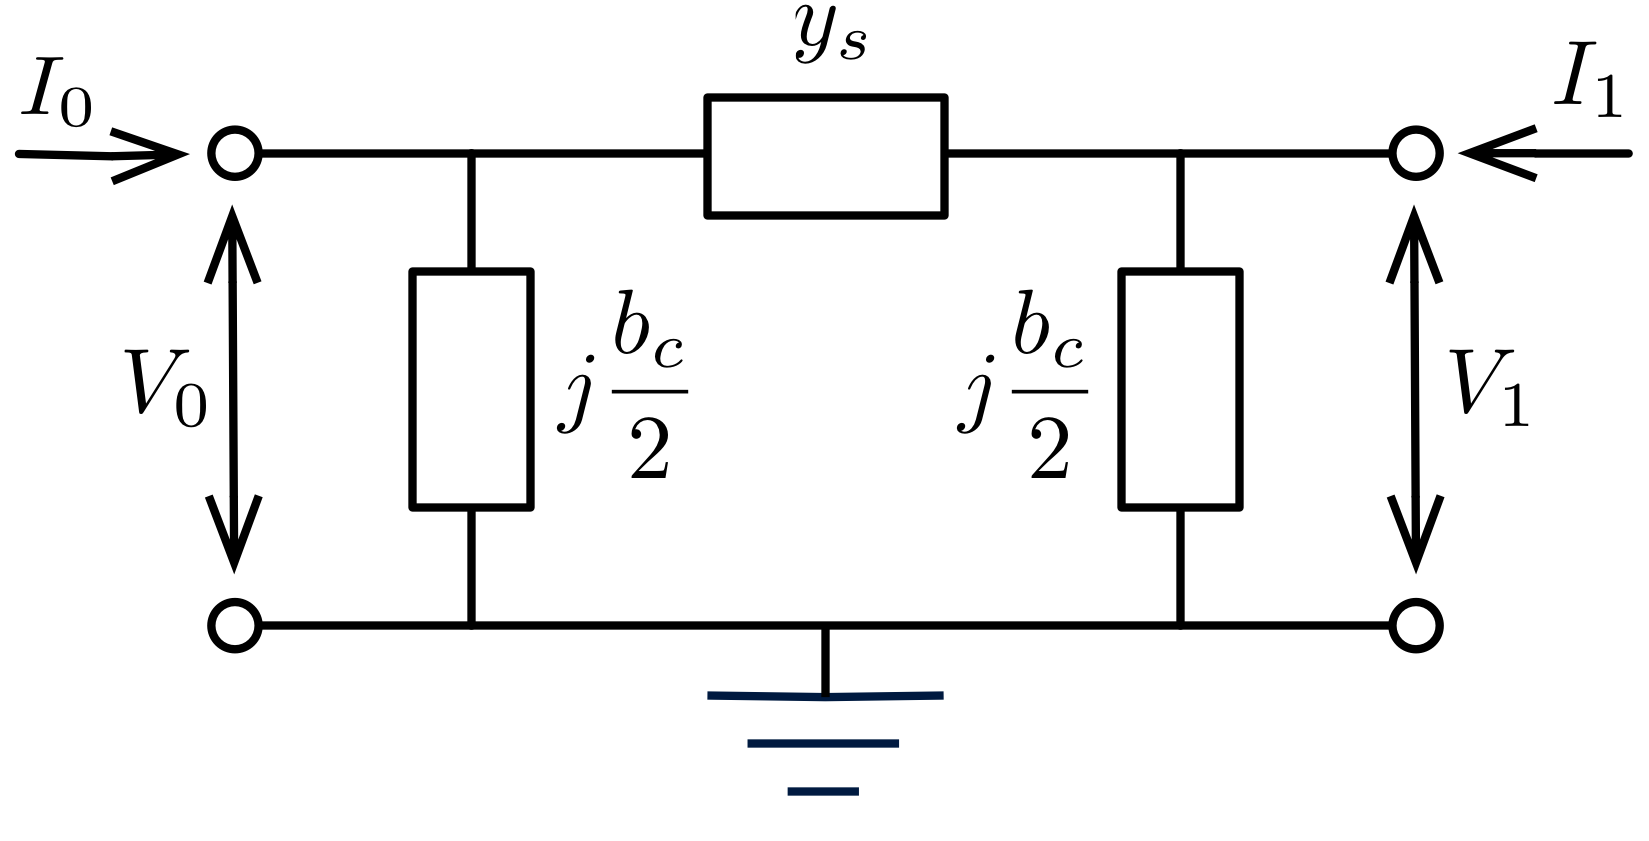
\includegraphics[width=(5cm)]{pi_line}
	\end{center}
	\caption{
		The $\pi$ model of a transmission line.
	}
	\label{FIG_PI_LINE}
\end{figure}
Very long lines require a more complex \emph{distributed model}.

\subsection{Multi-phase transmission lines}
The equations above apply also to multi-phase lines, except that the scalar elements become block submatrices whose size is the number of phases.

\subsection{Line parameters}
We have discussed above the structure of the $Y$ matrix for transmission lines -- but we still need to know how to find the values of the admittances in our equations. \emph{Carson's Equations} allow us to do this, for N-phase lines which may also contain one or more multi-grounded neutral wires. They take into account the geometry of the transmission line and the conductivity of the ground. We do not, however, go into these equations in this document.

\section{Transformers}
\subsection{Single phase transformers}
For an ideal transformer with a single (possibly complex) turns ratio $n = n_1/n_0$, we have, using the ABCD parameters:
\begin{align}
\begin{bmatrix}V_1 \\ I_1\end{bmatrix} &= \begin{bmatrix}n & 0 \\ 0 & 1/n^*\end{bmatrix}\begin{bmatrix}V_0 \\ I_0 \end{bmatrix}
\end{align}
This can't be modelled correctly in the formalism of nodal admittance matrices, in the same way that a line with zero impedance can't. Two equivalent circuits for an ideal transformer are shown in Fig. \ref{FIG_IDEAL_TRANS_EQUIV}.
\begin{figure}[!h]
	\begin{center}
		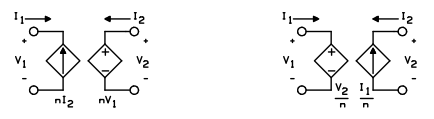
\includegraphics[width=(\textwidth-2cm)]{ideal_transformer_equiv.png}
	\end{center}
	\caption{
		Two equivalent circuits for an ideal transformer.
	}
	\label{FIG_IDEAL_TRANS_EQUIV}
\end{figure}
The relationships could be included in the powerflow equations specially, but more commonly real transformers are used, as described below; these may be expressed in the nodal admittance formalism.

A real transformer includes a leakage impedance (due to finite resistance of copper windings and core losses) and a shunt magnetising impedance. There are various ways of drawing an equivalent circuit. We use the general branch model described in Section \ref{SEC_GEN_BRANCH_MODEL}, see Fig. \ref{FIG_GEN_BRANCH_MODEL}.

The nodal admittance matrix is:
\begin{align}
\begin{bmatrix}I_0 \\ I_1 \end{bmatrix} &= 
\begin{bmatrix}\frac{y_l + \frac{1}{2}y_m}{|n|^2} & -\frac{y_l}{n^*} \\ -\frac{y_l}{n} & y_l + \frac{1}{2}y_m\end{bmatrix}
\begin{bmatrix}V_0 \\ V_1 \end{bmatrix}
\end{align}
where $n = n_1/n_0$ is the ideal turns ratio, $y_l$ is the leakage impedance and $y_m$ is the magnetising admittance. Often, the magnetising admittance is very small and is neglected. $y_l$ can be found by short circuiting the secondary, while $y_m$ can be found using an open circuit test.

\subsection{Three-phase transformers}
The nodal admittance matrices of three-phase transformers may be derived from the single-phase expression, above, combined with information about the connections between phases.
\subsubsection{Delta-GWye}
\begin{figure}
\begin{center}
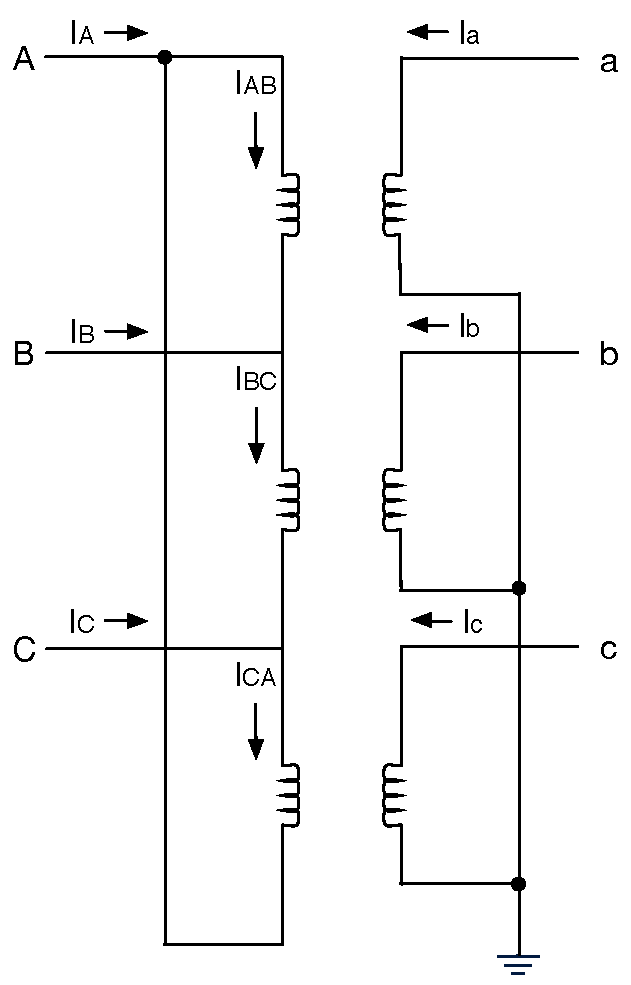
\includegraphics[width=7cm]{DeltaGWye.pdf}
\caption{Schematic of a Delta-GWye transformer}
\label{FIG_DELTA_GWYE}
\end{center}
\end{figure}
Considering Fig. \ref{FIG_DELTA_GWYE} and neglecting the magnetising impedance, we have,
\begin{align}
I_{AB} &= \frac{y_l}{|n|^2}(V_A - V_B) - \frac{y_l}{n^*}V_a \\
I_{BC} &= \frac{y_l}{|n|^2}(V_B - V_C) - \frac{y_l}{n^*}V_b \\
I_{CA} &= \frac{y_l}{|n|^2}(V_C - V_A) - \frac{y_l}{n^*}V_c \\
I_a &= -\frac{y_l}{n}(V_A - V_B) + y_l V_a \\
I_b &= -\frac{y_l}{n}(V_B - V_C) + y_l V_b \\
I_c &= -\frac{y_l}{n}(V_C - V_A) + y_l V_c \\
\end{align}
Also, by the KCL, we have
\begin{align}
I_A &= I_{AB} - I_{CA} \\
&= \frac{y_l}{|n|^2}(2V_A - V_B - V_C) + \frac{y_l}{n^*}(V_c - V_a) \\
I_B &= I_{BC} - I_{AB} \\
&= \frac{y_l}{|n|^2}(2V_B - V_C - V_A) + \frac{y_l}{n^*}(V_a - V_b) \\
I_C &= I_{CA} - I_{BC} \\
&= \frac{y_l}{|n|^2}(2V_C - V_A - V_B) + \frac{y_l}{n^*}(V_b - V_c)
\end{align}
so we can immediately write down the nodal admittance relationship:
\begin{align}
\begin{bmatrix}I_A \\ I_B \\ I_C \\ I_a \\ I_b \\ I_c\end{bmatrix} &=
y_l \begin{bmatrix}
	2/|n|^2 & -1/|n|^2 & -1/|n|^2 & -1/n^* & 0 & 1/n^* \\
	-1/|n|^2 & 2/|n|^2 &  -1/|n|^2 & 1/n^*  & -1/n^* & 0 \\
	-1/|n|^2 &  -1/|n|^2 & 2/|n|^2 & 0 & 1/n^*  & -1/n^* \\
	-1/n & 1/n & 0 & 1 & 0 & 0 \\
	0 & -1/n & 1/n & 0 & 1 & 0 \\
	1/n & 0 & -1/n & 0 & 0 & 1
\end{bmatrix}
\begin{bmatrix}V_A \\ V_B \\ V_C \\ V_a \\ V_b \\ V_c\end{bmatrix}
\end{align}
with the nodal admittance matrix being specified by the matrix on the right, including the factor of $y_l$.

\section{General single phase branch model}
\label{SEC_GEN_BRANCH_MODEL}
Single phase transformers and transmission lines can both be incorporated within a single general branch model, shown in Fig. \ref{FIG_GEN_BRANCH_MODEL}.
\begin{figure}[!h]
	\begin{center}
		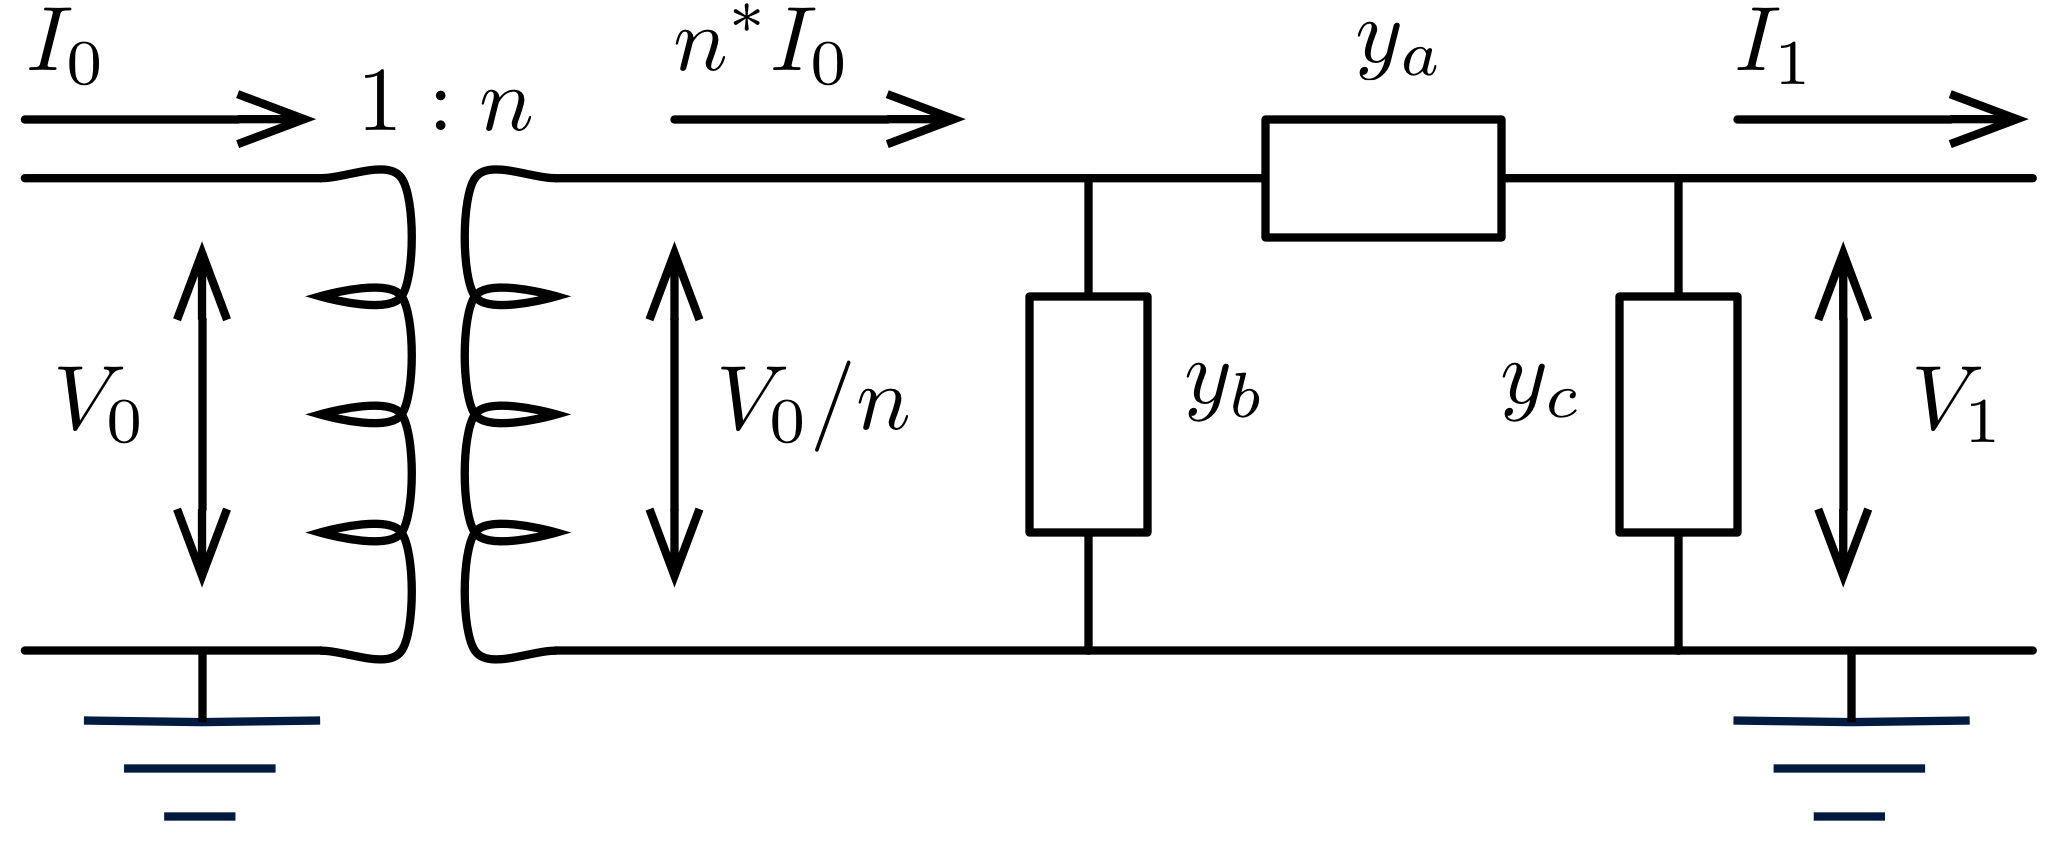
\includegraphics[width=(9cm)]{branch.png}
	\end{center}
	\caption{
		A general branch model, similar but more general than that used by {\sc Matpower}.
	}
	\label{FIG_GEN_BRANCH_MODEL}
\end{figure}
The $Y$ matrix for this model is defined by the following equation:
\begin{align}
	\begin{bmatrix}I_0 \\ I_1\end{bmatrix} &=
	\begin{bmatrix}\frac{y_a + y_b}{|n|^2} & -\frac{y_a}{n^*} \\ -\frac{y_a}{n} & y_a + y_c \end{bmatrix}
	\begin{bmatrix}V_0 \\ V_1\end{bmatrix}
\end{align}
Normally, $y_b = y_c = -jb_c/2$ for both transformers and transmission lines, as per the {\sc Matpower} manual. For a transmission line, $b_c$ is a capacitative admittance, and is positive, and for a transformer, $b_c$ is an inductive admittance and is negative. For both transformers and lines, $y_a$ has a real positive part (corresponding to the resistance) and a negative imaginary part (an inductive admittance).

\section{Units and the per-unit system}
The following self-consistent system of units is often used in modelling electricity networks:
\begin{description}
	\item[Voltage:]kV (kilovolts)
	\item[Power:]MW/MVAR/MVA (megawatts etc.)
	\item[Current:]kA (kiloamps)
	\item[Resistance:]$\Omega$ (ohms)
	\item[Admittance:]$S$ (siemens)
\end{description}
Under this system, relationships like Ohm's Law hold without the need to include any additional constants. The alternative is to use SI units ($V/W/A/\Omega/S$\ldots).

The \emph{per-unit} system is also often used. The idea is to express electrical quantities as a \emph{per-unit} dimensionless quantity times a \emph{base unit}, e.g.
\begin{align}
V &= V_\text{pu}V_\text{base} \notag \\
S &= S_\text{pu}P_\text{base} \notag \\
I &= I_\text{pu}I_\text{base} \notag \\
&\text{etc.}
\end{align}

Base units $V_\text{base}$ and $P_\text{base}$ are normally first defined for the network. $V_\text{base}$ is set to the nominal operating voltage of a bus (e.g. 11~kV), which means that $V_\text{base}$ may vary from bus to bus. On the other hand, a single network-wide value for $P_\text{base}$ is usually chosen to be a convenient value such as 100~MVA. Other base quantities may then be derived:
\begin{align}
	I_\text{base} &= P_\text{base}/V_\text{base} \notag \\
	Z_\text{base} &= V_\text{base}^2 / P_\text{base} \notag \\
	Y_\text{base} &= P_\text{base} / V_\text{base}^2
\end{align}
Note that there is some ambiguity about which bus $V_\text{base}$ is referenced to in the expressions above. Consider for example a line that runs between two busses: logically there could be several ways to define the per-unit current: using the voltage at the first bus, the voltage at the second bus, or the voltage drop on the line. Depending on how things are done, different equations will need to be used for the network. A set of conventions consistent with \textsc{Matpower} is given below:
\begin{itemize}
\item Per-unit quantities in lines are calculated using the base-voltage at the second (to) bus. This makes sense in Matpower, since a common branch model is used where all transformers occur at the first (from) bus, with the bulk of the line occurring between the transformer and the second (to) bus.
\item Per-unit quantities associated with busses (such as bus shunt admittance, current loads etc. are calculated, naturally enough, using the base voltage of the bus.
\end{itemize}

\section{The Swing Equations}
A synchronous generator has a flywheel with moment of inertia $J$. There is a mechanical torque (e.g. from the turbine) $T_m$ pushing the rotor and an electrical torque $T_e$ that comes from the alternator and usually acts against the mechanical torque. We define the torque imbalance $\Delta T = T_m - T_e$. When $\Delta T$ is positive the rotor will speed up and when it is negative it will slow down. We define the rotor angle $\theta$ which is assumed to be zero at $t = 0$. Its first time derivative is the angular velocity $\omega = \dot{\theta}$.

The equation \footnote{For those not familiar with the notation, a dot above a variable indicates a time derivative, e.g. $\dot{\theta} := \partial \theta / \partial t$. Similarly, a double dot indicates a second time derivative, etc.} governing the motion of the rotor is
\begin{align}
	J \ddot{\theta} &= \Delta T
\end{align}
which is analogous to Newton's $F = ma$.

For a rotor running at the constant mandated network angular frequency $\omega_\text{nom}$, we have $\theta = \omega_\text{nom} t$. Because the rotor may deviate from this frequency, we define the angular error
\begin{align}
	\Delta \theta &= \theta - \omega_\text{nom} t. \label{EQ_DEFN_DELTA_THETA}
\end{align}
This quantity is basically equal to the voltage phase of the generator internal bus. In terms of this new variable, the generator equation is:
\begin{align}
	J \Delta \ddot{\theta} &= \Delta T
\end{align}

Since the power $P = \omega T$, we multiply both sides of the second equation by $\omega$ to obtain a relation for the power mismatch:
\begin{align}
	J\omega \Delta \ddot{\theta} &= \Delta P \notag \\
	J\left(\omega_\text{nom} + \Delta \dot{\theta}\right) \Delta\ddot{\theta} &= \Delta P
\end{align}
where $\Delta P$ is the input mechanical power minus the electrical power supplied to the network. When the rotor is running far from the mandated frequency, then this equation would need to be applied as is. However, at frequencies near the network frequency, $\omega_\text{nom} \gg \dot{\theta}$, and so we can write
\begin{align}
	J\omega_\text{nom} \Delta\ddot{\theta} &= L_\text{nom} \Delta\ddot{\theta} = \Delta P \label{EQ_SWING}
\end{align}
where $L_\text{nom} = J \omega_\text{nom}$ is the angular momentum of the rotor at the network frequency. This is the swing equation, and when solved will give the bus internal voltage angle as a function of time.

A note about units: if, as is common, we measure power in $\mathrm{MVA}$, then $L$ will need to be measured in commensurate units of $\mathrm{Mkg\cdot m^{-2}}$, i.e. we will need to divide the SI value by $10^6$.

\subsection{Multiple-pole generators}
Generators may have multiple pairs of north-south magnetic dipoles. In such cases, the rotor angular frequency will be scaled with respect to the network frequency. For example, a generator with two dipoles running on a 50~Hz network will turn at 25~Hz, because the north-south fields will pass the coils at twice the rate of the rotor's rotation.

Such cases are easily taken care of by absorbing the scaling factor into $J$.

\subsection{The Velocity Verlet algorithm}
A good way of solving such kinds of equations of motion is the Velocity Verlet algorithm, often used in molecular dynamics simulation. Note that $\Delta P$ is normally dependent only on the instantaneous properties of the network including the voltage angle $\delta$. This algorithm has the advantage of being \emph{symplectic}, meaning effectively that it has the property of time reversibility, that spurious energies are not added to the system and therefore we do not see the kinds of instabilities that give rise to wild and spurious accelerations.

The steps in the algorithm are given below. We put $\omega_\delta := \partial \delta / \partial t$ and $\alpha_\delta := \partial^2 \delta / \partial t^2$
\begin{enumerate}
	\item $\delta(t + \Delta t) = \delta(t) + \omega_\delta\Delta t + \frac{1}{2}\alpha_\delta\Delta t^2$,
	\item Derive $\alpha_\delta(t + \Delta t)$. First calculate $\Delta P(t + \Delta t) = P_m(t + \Delta t) - P_e(\delta(t + \Delta t))$. $P_m$ is a known function of time, and $P_e$ is found by solving the AC power flow equations, using the calculated phase angles $\delta(t + \Delta t)$ for all generators. Then, from the swing equation, Eq. \ref{EQ_SWING}, we have $\alpha_\delta(t + \Delta t) = \Delta P(t + \Delta t)/L_\text{nom}$
	\item $\omega_\delta(t + \Delta t) = \omega_\delta(t) + \frac{1}{2}\left[\alpha_\delta(t + \Delta t) + \alpha_\delta(t)\right]\Delta t$
\end{enumerate}

\subsection{The swing equations and the power flow equations}
In step 2 above, we derive the electrical power at all generators using the power flow equations. We need to specify the exact form of the equations used. The first observation is that the phase angle $\phi$ is fixed at the generator busses by the swing equations. The voltage magnitude $V$ could also be fixed (either to its fixed value, or scaled according to the current frequency), making all of the busses into effective swing busses. To ensure feasibility of the AC power flow equations, we could then convert all or some ZIP loads into constant impedance loads, or add a high constant impedance component to all loads to ensure feasibility.

Note that for the purposes of the swing equations, we are only interested in the real power component of the power flow equations. However, to find this, we need all components of the voltage at all other busses, so solving a general power flow problem is necessary.

\subsection{The swing equations at a three phase bus}
We also need to consider how to handle things at a three phase bus. The three terminals of the bus are connected to a single rotor, with a given angular momentum. The phase relationship between the bus terminals is enforced by the windings in the stator. The problem is what to do with this situation, in regards to the swing equations etc.

The answer is the obvious: that there is a single machine at each generator, which is input for the swing equations. 

\end{document}